% Solar-powered acoustic monitoring of the endangered Houston toad.
% Preview: pdflatex research_frog.tex
% SVG:     latex -jobname=research_frog "\def\pgfsysdriver{pgfsys-dvisvgm.def}% Solar-powered acoustic monitoring of the endangered Houston toad.
% Preview: pdflatex research_frog.tex
% SVG:     latex -jobname=research_frog "\def\pgfsysdriver{pgfsys-dvisvgm.def}% Solar-powered acoustic monitoring of the endangered Houston toad.
% Preview: pdflatex research_frog.tex
% SVG:     latex -jobname=research_frog "\def\pgfsysdriver{pgfsys-dvisvgm.def}% Solar-powered acoustic monitoring of the endangered Houston toad.
% Preview: pdflatex research_frog.tex
% SVG:     latex -jobname=research_frog "\def\pgfsysdriver{pgfsys-dvisvgm.def}\input{research_frog}"
%          dvisvgm --no-fonts --exact-bbox --optimize research_frog.dvi
\documentclass[tikz,border=0pt]{standalone}
\usepackage[T1]{fontenc}
\usepackage{lmodern}
\usepackage{amsmath}
\usetikzlibrary{arrows.meta,backgrounds}

\definecolor{ink}{HTML}{1F2328}
\definecolor{mute}{HTML}{59636E}
\definecolor{faint}{HTML}{8C959F}
\definecolor{rule}{HTML}{D0D7DE}
\definecolor{call}{HTML}{8E1B3A}
\definecolor{ochre}{HTML}{C08A2E}
\definecolor{slate}{HTML}{2F5C8A}
\definecolor{ml}{HTML}{0F766E}
\definecolor{reed}{HTML}{B8A398}

\begin{document}
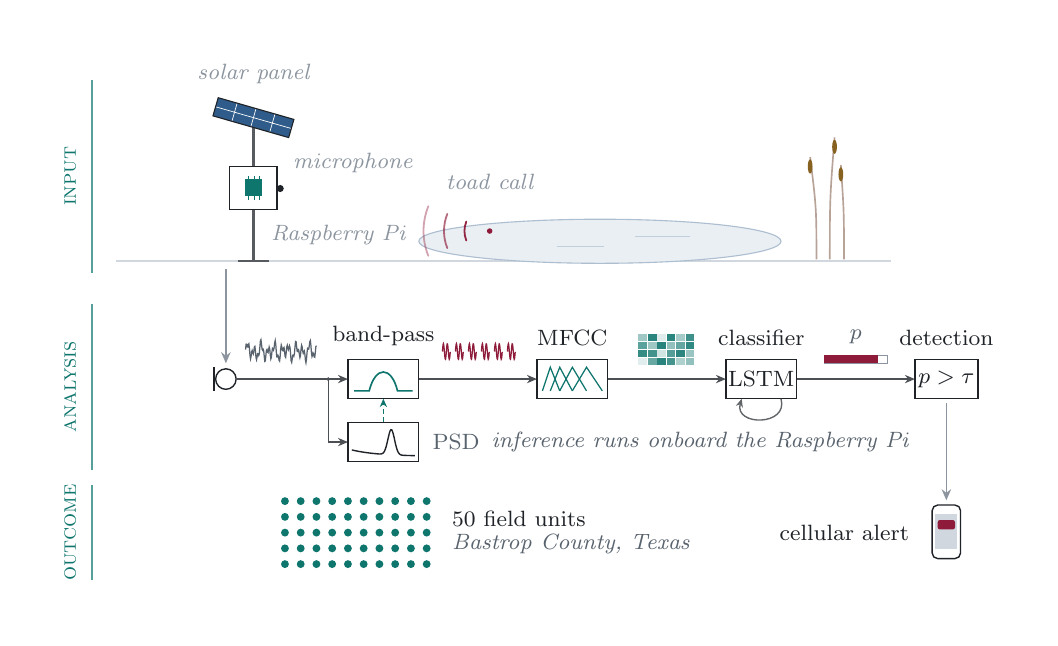
\begin{tikzpicture}[
    font=\footnotesize, text=ink,
    show background rectangle,
    background rectangle/.style={fill=white},
    inner frame sep=10pt,
    tag/.style={text=faint, font=\footnotesize\itshape},
    note/.style={text=mute, font=\footnotesize\itshape},
    region/.style={text=ml, font=\footnotesize\scshape, rotate=90, anchor=south},
    blk/.style={draw=ink, line width=0.5pt, fill=white},
    wire/.style={draw=ink!80, line width=0.55pt, -{Stealth[length=3.6pt, width=3pt]}},
    flow/.style={draw=faint, line width=0.6pt, -{Stealth[length=4pt, width=3.4pt]}}]

  % ----------------------------------------------------------- tiers
  \foreach \ya/\yb/\t in {4.45/6.90/input, 1.95/4.05/analysis, 0.55/1.75/outcome} {
    \draw[ml!70, line width=0.5pt] (-0.05,\ya) -- (-0.05,\yb);
    \node[region] at (-0.13,{(\ya+\yb)/2}) {\t};
  }

  % ------------------------------------------- input: field recording
  \draw[rule, line width=0.5pt] (0.25,4.60) -- (10.10,4.60);
  \draw[ink!75, line width=1.2pt] (2.00,4.60) -- (2.00,6.30);
  \draw[ink!75, line width=0.6pt] (1.80,4.60) -- (2.20,4.60);
  \fill[white] (1.70,5.25) rectangle (2.30,5.80);
  \draw[ink, line width=0.45pt] (1.70,5.25) rectangle (2.30,5.80);
  \fill[ml] (1.89,5.42) rectangle (2.11,5.64);
  \foreach \t in {0.05,0.12,0.19}
    \draw[ml, line width=0.3pt] (1.89+\t,5.42) -- ++(0,-0.04) (1.89+\t,5.64) -- ++(0,0.04);
  \fill[ink] (2.34,5.52) circle (0.045);
  \begin{scope}[shift={(2.00,6.42)}, rotate=-16]
    \fill[slate] (-0.50,-0.12) rectangle (0.50,0.12);
    \draw[white, line width=0.25pt] (-0.25,-0.12) -- (-0.25,0.12) (0,-0.12) -- (0,0.12)
      (0.25,-0.12) -- (0.25,0.12) (-0.50,0) -- (0.50,0);
    \draw[ink, line width=0.4pt] (-0.50,-0.12) rectangle (0.50,0.12);
  \end{scope}
  \fill[slate!10] (6.40,4.85) ellipse[x radius=2.30, y radius=0.28];
  \draw[slate!40, line width=0.4pt] (6.40,4.85) ellipse[x radius=2.30, y radius=0.28];
  \draw[slate!30, line width=0.35pt] (5.85,4.79) -- (6.45,4.79) (6.85,4.91) -- (7.55,4.91);
  \foreach \x/\h/\b in {9.15/1.30/-8, 9.32/1.55/6, 9.50/1.20/-4} {
    \draw[reed, line width=0.6pt] (\x,4.62) .. controls (\x,{4.62+0.5*\h}) .. ({\x+\b*0.01},{4.62+\h});
    \fill[ochre!70!black] ({\x+\b*0.01},{4.50+\h}) ellipse[x radius=0.03, y radius=0.09];
  }
  \foreach \r/\o in {0.32/0.95, 0.58/0.65, 0.84/0.40}
    \draw[call, line width=0.65pt, opacity=\o, line cap=round]
      (5.00,4.98) ++(158:\r) arc[start angle=158, end angle=202, radius=\r];
  \fill[call] (5.00,4.98) circle (0.035);
  \node[tag, anchor=south] at (5.00,5.38) {toad call};
  \node[tag, anchor=south] at (2.00,6.72) {solar panel};
  \node[tag, anchor=south west] at (2.38,5.60) {microphone};
  \node[tag, anchor=north west] at (2.10,5.18) {Raspberry Pi};

  \draw[flow] (1.65,4.50) -- (1.65,3.30);

  % --------------------------------------- analysis: onboard pipeline
  \draw[ink, line width=0.5pt] (1.65,3.10) circle (0.13);
  \draw[ink, line width=0.9pt] (1.50,2.95) -- (1.50,3.25);
  \draw[wire] (1.78,3.10) -- (3.20,3.10);
  \draw[mute, line width=0.45pt] plot[domain=0:0.9, samples=130]
    ({1.90+\x},{3.45+0.07*sin(4100*\x)+0.05*sin(9700*\x+30)+0.04*sin(2300*\x)});
  \fill[ink!80] (2.95,3.10) circle (0.025);
  \draw[ink!80, line width=0.5pt] (2.95,3.10) -- (2.95,2.30);
  \draw[wire] (2.95,2.30) -- (3.20,2.30);

  \draw[blk] (3.20,2.05) rectangle (4.10,2.55);                               % PSD
  \draw[ink, line width=0.5pt] plot[domain=0:0.8, samples=80]
    ({3.25+\x},{2.12+0.32*exp(-pow((\x-0.5)/0.06,2))+0.08*exp(-3*\x)});
  \node[anchor=west, text=mute] at (4.15,2.30) {PSD};
  \draw[ml, line width=0.5pt, dash pattern=on 1.8pt off 1.4pt, -{Stealth[length=3pt, width=2.6pt]}]
    (3.65,2.55) -- (3.65,2.85);

  \draw[blk] (3.20,2.85) rectangle (4.10,3.35);                               % band-pass
  \draw[ml, line width=0.6pt] (3.28,2.95) -- (3.47,2.95) .. controls (3.55,3.27) and (3.75,3.27) .. (3.83,2.95) -- (4.02,2.95);
  \node[anchor=south] at (3.65,3.40) {band-pass};
  \draw[wire] (4.10,3.10) -- (5.60,3.10);
  \foreach \k in {0,...,5}
    \draw[call, line width=0.45pt] plot[domain=0:0.1, samples=24] ({4.40+0.165*\k+\x},{3.45+0.10*sin(7200*\x)});

  \draw[blk] (5.60,2.85) rectangle (6.50,3.35);                               % MFCC
  \foreach \a/\b/\c in {5.67/5.77/5.89, 5.77/5.89/6.05, 5.89/6.05/6.23, 6.05/6.23/6.43}
    \draw[ml, line width=0.45pt] (\a,2.95) -- (\b,3.25) -- (\c,2.95);
  \node[anchor=south] at (6.05,3.40) {MFCC};
  \draw[wire] (6.50,3.10) -- (8.00,3.10);
  \foreach \i in {0,...,5} \foreach \j in {0,...,3} {
    \pgfmathsetmacro\o{0.12+0.78*abs(sin(41*\i+67*\j+13*\i*\j))}
    \fill[ml, opacity=\o] (6.89+0.12*\i,3.28+0.10*\j) rectangle ++(0.11,0.09);
  }

  \draw[blk] (8.00,2.85) rectangle (8.90,3.35);                               % LSTM
  \node at (8.45,3.10) {LSTM};
  \draw[ink!70, line width=0.5pt, -{Stealth[length=3pt, width=2.6pt]}]
    (8.70,2.85) .. controls (8.80,2.50) and (8.10,2.50) .. (8.20,2.85);
  \node[anchor=south] at (8.45,3.40) {classifier};
  \draw[wire] (8.90,3.10) -- (10.40,3.10);
  \draw[faint, line width=0.4pt] (9.25,3.30) rectangle (10.05,3.40);
  \fill[call] (9.25,3.30) rectangle (9.93,3.40);
  \node[anchor=south, text=mute] at (9.65,3.42) {$p$};

  \draw[blk] (10.40,2.85) rectangle (11.20,3.35);                             % decision
  \node at (10.80,3.10) {$p > \tau$};
  \node[anchor=south] at (10.80,3.40) {detection};
  \node[note, anchor=west] at (4.90,2.30) {inference runs onboard the Raspberry Pi};

  \draw[flow] (10.80,2.80) -- (10.80,1.56);

  % ------------------------------------------------ outcome: alerts
  \draw[ink, line width=0.5pt, rounded corners=2pt, fill=white] (10.62,0.82) rectangle (10.98,1.50);
  \fill[rule] (10.66,0.94) rectangle (10.94,1.38);
  \fill[call, rounded corners=0.8pt] (10.69,1.19) rectangle (10.91,1.31);
  \node[anchor=east] at (10.45,1.15) {cellular alert};
  \foreach \i in {0,...,9} \foreach \j in {0,...,4}
    \fill[ml] (2.40+0.20*\i,0.75+0.20*\j) circle (0.05);
  \node[anchor=west, align=left] at (4.40,1.15) {50 field units\\[-1pt]\textcolor{mute}{\itshape Bastrop County, Texas}};
\end{tikzpicture}
\end{document}
"
%          dvisvgm --no-fonts --exact-bbox --optimize research_frog.dvi
\documentclass[tikz,border=0pt]{standalone}
\usepackage[T1]{fontenc}
\usepackage{lmodern}
\usepackage{amsmath}
\usetikzlibrary{arrows.meta,backgrounds}

\definecolor{ink}{HTML}{1F2328}
\definecolor{mute}{HTML}{59636E}
\definecolor{faint}{HTML}{8C959F}
\definecolor{rule}{HTML}{D0D7DE}
\definecolor{call}{HTML}{8E1B3A}
\definecolor{ochre}{HTML}{C08A2E}
\definecolor{slate}{HTML}{2F5C8A}
\definecolor{ml}{HTML}{0F766E}
\definecolor{reed}{HTML}{B8A398}

\begin{document}
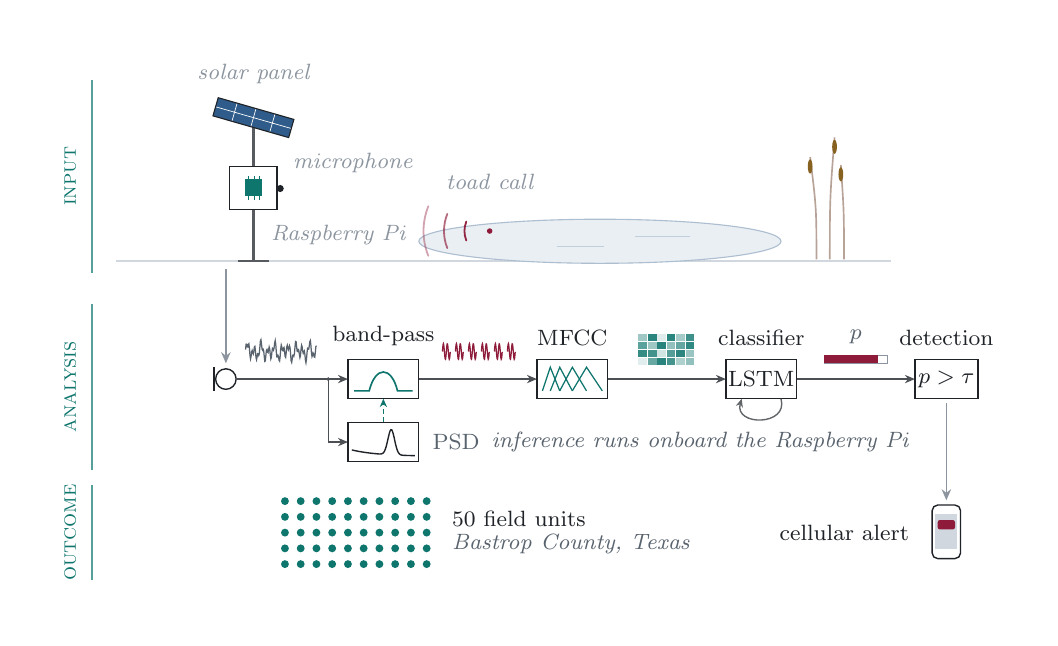
\begin{tikzpicture}[
    font=\footnotesize, text=ink,
    show background rectangle,
    background rectangle/.style={fill=white},
    inner frame sep=10pt,
    tag/.style={text=faint, font=\footnotesize\itshape},
    note/.style={text=mute, font=\footnotesize\itshape},
    region/.style={text=ml, font=\footnotesize\scshape, rotate=90, anchor=south},
    blk/.style={draw=ink, line width=0.5pt, fill=white},
    wire/.style={draw=ink!80, line width=0.55pt, -{Stealth[length=3.6pt, width=3pt]}},
    flow/.style={draw=faint, line width=0.6pt, -{Stealth[length=4pt, width=3.4pt]}}]

  % ----------------------------------------------------------- tiers
  \foreach \ya/\yb/\t in {4.45/6.90/input, 1.95/4.05/analysis, 0.55/1.75/outcome} {
    \draw[ml!70, line width=0.5pt] (-0.05,\ya) -- (-0.05,\yb);
    \node[region] at (-0.13,{(\ya+\yb)/2}) {\t};
  }

  % ------------------------------------------- input: field recording
  \draw[rule, line width=0.5pt] (0.25,4.60) -- (10.10,4.60);
  \draw[ink!75, line width=1.2pt] (2.00,4.60) -- (2.00,6.30);
  \draw[ink!75, line width=0.6pt] (1.80,4.60) -- (2.20,4.60);
  \fill[white] (1.70,5.25) rectangle (2.30,5.80);
  \draw[ink, line width=0.45pt] (1.70,5.25) rectangle (2.30,5.80);
  \fill[ml] (1.89,5.42) rectangle (2.11,5.64);
  \foreach \t in {0.05,0.12,0.19}
    \draw[ml, line width=0.3pt] (1.89+\t,5.42) -- ++(0,-0.04) (1.89+\t,5.64) -- ++(0,0.04);
  \fill[ink] (2.34,5.52) circle (0.045);
  \begin{scope}[shift={(2.00,6.42)}, rotate=-16]
    \fill[slate] (-0.50,-0.12) rectangle (0.50,0.12);
    \draw[white, line width=0.25pt] (-0.25,-0.12) -- (-0.25,0.12) (0,-0.12) -- (0,0.12)
      (0.25,-0.12) -- (0.25,0.12) (-0.50,0) -- (0.50,0);
    \draw[ink, line width=0.4pt] (-0.50,-0.12) rectangle (0.50,0.12);
  \end{scope}
  \fill[slate!10] (6.40,4.85) ellipse[x radius=2.30, y radius=0.28];
  \draw[slate!40, line width=0.4pt] (6.40,4.85) ellipse[x radius=2.30, y radius=0.28];
  \draw[slate!30, line width=0.35pt] (5.85,4.79) -- (6.45,4.79) (6.85,4.91) -- (7.55,4.91);
  \foreach \x/\h/\b in {9.15/1.30/-8, 9.32/1.55/6, 9.50/1.20/-4} {
    \draw[reed, line width=0.6pt] (\x,4.62) .. controls (\x,{4.62+0.5*\h}) .. ({\x+\b*0.01},{4.62+\h});
    \fill[ochre!70!black] ({\x+\b*0.01},{4.50+\h}) ellipse[x radius=0.03, y radius=0.09];
  }
  \foreach \r/\o in {0.32/0.95, 0.58/0.65, 0.84/0.40}
    \draw[call, line width=0.65pt, opacity=\o, line cap=round]
      (5.00,4.98) ++(158:\r) arc[start angle=158, end angle=202, radius=\r];
  \fill[call] (5.00,4.98) circle (0.035);
  \node[tag, anchor=south] at (5.00,5.38) {toad call};
  \node[tag, anchor=south] at (2.00,6.72) {solar panel};
  \node[tag, anchor=south west] at (2.38,5.60) {microphone};
  \node[tag, anchor=north west] at (2.10,5.18) {Raspberry Pi};

  \draw[flow] (1.65,4.50) -- (1.65,3.30);

  % --------------------------------------- analysis: onboard pipeline
  \draw[ink, line width=0.5pt] (1.65,3.10) circle (0.13);
  \draw[ink, line width=0.9pt] (1.50,2.95) -- (1.50,3.25);
  \draw[wire] (1.78,3.10) -- (3.20,3.10);
  \draw[mute, line width=0.45pt] plot[domain=0:0.9, samples=130]
    ({1.90+\x},{3.45+0.07*sin(4100*\x)+0.05*sin(9700*\x+30)+0.04*sin(2300*\x)});
  \fill[ink!80] (2.95,3.10) circle (0.025);
  \draw[ink!80, line width=0.5pt] (2.95,3.10) -- (2.95,2.30);
  \draw[wire] (2.95,2.30) -- (3.20,2.30);

  \draw[blk] (3.20,2.05) rectangle (4.10,2.55);                               % PSD
  \draw[ink, line width=0.5pt] plot[domain=0:0.8, samples=80]
    ({3.25+\x},{2.12+0.32*exp(-pow((\x-0.5)/0.06,2))+0.08*exp(-3*\x)});
  \node[anchor=west, text=mute] at (4.15,2.30) {PSD};
  \draw[ml, line width=0.5pt, dash pattern=on 1.8pt off 1.4pt, -{Stealth[length=3pt, width=2.6pt]}]
    (3.65,2.55) -- (3.65,2.85);

  \draw[blk] (3.20,2.85) rectangle (4.10,3.35);                               % band-pass
  \draw[ml, line width=0.6pt] (3.28,2.95) -- (3.47,2.95) .. controls (3.55,3.27) and (3.75,3.27) .. (3.83,2.95) -- (4.02,2.95);
  \node[anchor=south] at (3.65,3.40) {band-pass};
  \draw[wire] (4.10,3.10) -- (5.60,3.10);
  \foreach \k in {0,...,5}
    \draw[call, line width=0.45pt] plot[domain=0:0.1, samples=24] ({4.40+0.165*\k+\x},{3.45+0.10*sin(7200*\x)});

  \draw[blk] (5.60,2.85) rectangle (6.50,3.35);                               % MFCC
  \foreach \a/\b/\c in {5.67/5.77/5.89, 5.77/5.89/6.05, 5.89/6.05/6.23, 6.05/6.23/6.43}
    \draw[ml, line width=0.45pt] (\a,2.95) -- (\b,3.25) -- (\c,2.95);
  \node[anchor=south] at (6.05,3.40) {MFCC};
  \draw[wire] (6.50,3.10) -- (8.00,3.10);
  \foreach \i in {0,...,5} \foreach \j in {0,...,3} {
    \pgfmathsetmacro\o{0.12+0.78*abs(sin(41*\i+67*\j+13*\i*\j))}
    \fill[ml, opacity=\o] (6.89+0.12*\i,3.28+0.10*\j) rectangle ++(0.11,0.09);
  }

  \draw[blk] (8.00,2.85) rectangle (8.90,3.35);                               % LSTM
  \node at (8.45,3.10) {LSTM};
  \draw[ink!70, line width=0.5pt, -{Stealth[length=3pt, width=2.6pt]}]
    (8.70,2.85) .. controls (8.80,2.50) and (8.10,2.50) .. (8.20,2.85);
  \node[anchor=south] at (8.45,3.40) {classifier};
  \draw[wire] (8.90,3.10) -- (10.40,3.10);
  \draw[faint, line width=0.4pt] (9.25,3.30) rectangle (10.05,3.40);
  \fill[call] (9.25,3.30) rectangle (9.93,3.40);
  \node[anchor=south, text=mute] at (9.65,3.42) {$p$};

  \draw[blk] (10.40,2.85) rectangle (11.20,3.35);                             % decision
  \node at (10.80,3.10) {$p > \tau$};
  \node[anchor=south] at (10.80,3.40) {detection};
  \node[note, anchor=west] at (4.90,2.30) {inference runs onboard the Raspberry Pi};

  \draw[flow] (10.80,2.80) -- (10.80,1.56);

  % ------------------------------------------------ outcome: alerts
  \draw[ink, line width=0.5pt, rounded corners=2pt, fill=white] (10.62,0.82) rectangle (10.98,1.50);
  \fill[rule] (10.66,0.94) rectangle (10.94,1.38);
  \fill[call, rounded corners=0.8pt] (10.69,1.19) rectangle (10.91,1.31);
  \node[anchor=east] at (10.45,1.15) {cellular alert};
  \foreach \i in {0,...,9} \foreach \j in {0,...,4}
    \fill[ml] (2.40+0.20*\i,0.75+0.20*\j) circle (0.05);
  \node[anchor=west, align=left] at (4.40,1.15) {50 field units\\[-1pt]\textcolor{mute}{\itshape Bastrop County, Texas}};
\end{tikzpicture}
\end{document}
"
%          dvisvgm --no-fonts --exact-bbox --optimize research_frog.dvi
\documentclass[tikz,border=0pt]{standalone}
\usepackage[T1]{fontenc}
\usepackage{lmodern}
\usepackage{amsmath}
\usetikzlibrary{arrows.meta,backgrounds}

\definecolor{ink}{HTML}{1F2328}
\definecolor{mute}{HTML}{59636E}
\definecolor{faint}{HTML}{8C959F}
\definecolor{rule}{HTML}{D0D7DE}
\definecolor{call}{HTML}{8E1B3A}
\definecolor{ochre}{HTML}{C08A2E}
\definecolor{slate}{HTML}{2F5C8A}
\definecolor{ml}{HTML}{0F766E}
\definecolor{reed}{HTML}{B8A398}

\begin{document}
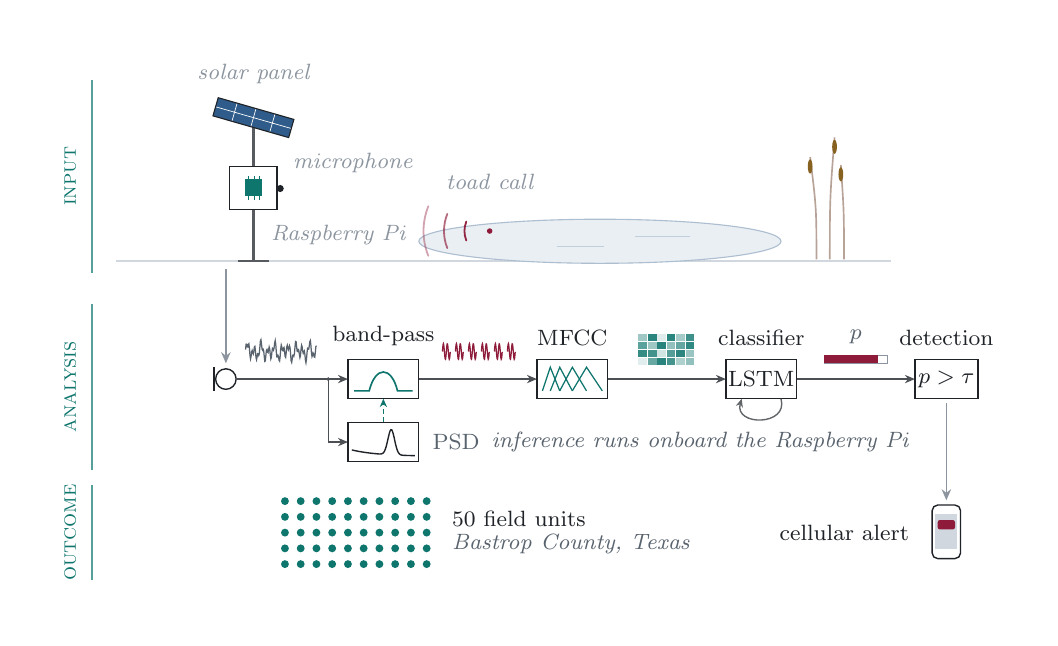
\begin{tikzpicture}[
    font=\footnotesize, text=ink,
    show background rectangle,
    background rectangle/.style={fill=white},
    inner frame sep=10pt,
    tag/.style={text=faint, font=\footnotesize\itshape},
    note/.style={text=mute, font=\footnotesize\itshape},
    region/.style={text=ml, font=\footnotesize\scshape, rotate=90, anchor=south},
    blk/.style={draw=ink, line width=0.5pt, fill=white},
    wire/.style={draw=ink!80, line width=0.55pt, -{Stealth[length=3.6pt, width=3pt]}},
    flow/.style={draw=faint, line width=0.6pt, -{Stealth[length=4pt, width=3.4pt]}}]

  % ----------------------------------------------------------- tiers
  \foreach \ya/\yb/\t in {4.45/6.90/input, 1.95/4.05/analysis, 0.55/1.75/outcome} {
    \draw[ml!70, line width=0.5pt] (-0.05,\ya) -- (-0.05,\yb);
    \node[region] at (-0.13,{(\ya+\yb)/2}) {\t};
  }

  % ------------------------------------------- input: field recording
  \draw[rule, line width=0.5pt] (0.25,4.60) -- (10.10,4.60);
  \draw[ink!75, line width=1.2pt] (2.00,4.60) -- (2.00,6.30);
  \draw[ink!75, line width=0.6pt] (1.80,4.60) -- (2.20,4.60);
  \fill[white] (1.70,5.25) rectangle (2.30,5.80);
  \draw[ink, line width=0.45pt] (1.70,5.25) rectangle (2.30,5.80);
  \fill[ml] (1.89,5.42) rectangle (2.11,5.64);
  \foreach \t in {0.05,0.12,0.19}
    \draw[ml, line width=0.3pt] (1.89+\t,5.42) -- ++(0,-0.04) (1.89+\t,5.64) -- ++(0,0.04);
  \fill[ink] (2.34,5.52) circle (0.045);
  \begin{scope}[shift={(2.00,6.42)}, rotate=-16]
    \fill[slate] (-0.50,-0.12) rectangle (0.50,0.12);
    \draw[white, line width=0.25pt] (-0.25,-0.12) -- (-0.25,0.12) (0,-0.12) -- (0,0.12)
      (0.25,-0.12) -- (0.25,0.12) (-0.50,0) -- (0.50,0);
    \draw[ink, line width=0.4pt] (-0.50,-0.12) rectangle (0.50,0.12);
  \end{scope}
  \fill[slate!10] (6.40,4.85) ellipse[x radius=2.30, y radius=0.28];
  \draw[slate!40, line width=0.4pt] (6.40,4.85) ellipse[x radius=2.30, y radius=0.28];
  \draw[slate!30, line width=0.35pt] (5.85,4.79) -- (6.45,4.79) (6.85,4.91) -- (7.55,4.91);
  \foreach \x/\h/\b in {9.15/1.30/-8, 9.32/1.55/6, 9.50/1.20/-4} {
    \draw[reed, line width=0.6pt] (\x,4.62) .. controls (\x,{4.62+0.5*\h}) .. ({\x+\b*0.01},{4.62+\h});
    \fill[ochre!70!black] ({\x+\b*0.01},{4.50+\h}) ellipse[x radius=0.03, y radius=0.09];
  }
  \foreach \r/\o in {0.32/0.95, 0.58/0.65, 0.84/0.40}
    \draw[call, line width=0.65pt, opacity=\o, line cap=round]
      (5.00,4.98) ++(158:\r) arc[start angle=158, end angle=202, radius=\r];
  \fill[call] (5.00,4.98) circle (0.035);
  \node[tag, anchor=south] at (5.00,5.38) {toad call};
  \node[tag, anchor=south] at (2.00,6.72) {solar panel};
  \node[tag, anchor=south west] at (2.38,5.60) {microphone};
  \node[tag, anchor=north west] at (2.10,5.18) {Raspberry Pi};

  \draw[flow] (1.65,4.50) -- (1.65,3.30);

  % --------------------------------------- analysis: onboard pipeline
  \draw[ink, line width=0.5pt] (1.65,3.10) circle (0.13);
  \draw[ink, line width=0.9pt] (1.50,2.95) -- (1.50,3.25);
  \draw[wire] (1.78,3.10) -- (3.20,3.10);
  \draw[mute, line width=0.45pt] plot[domain=0:0.9, samples=130]
    ({1.90+\x},{3.45+0.07*sin(4100*\x)+0.05*sin(9700*\x+30)+0.04*sin(2300*\x)});
  \fill[ink!80] (2.95,3.10) circle (0.025);
  \draw[ink!80, line width=0.5pt] (2.95,3.10) -- (2.95,2.30);
  \draw[wire] (2.95,2.30) -- (3.20,2.30);

  \draw[blk] (3.20,2.05) rectangle (4.10,2.55);                               % PSD
  \draw[ink, line width=0.5pt] plot[domain=0:0.8, samples=80]
    ({3.25+\x},{2.12+0.32*exp(-pow((\x-0.5)/0.06,2))+0.08*exp(-3*\x)});
  \node[anchor=west, text=mute] at (4.15,2.30) {PSD};
  \draw[ml, line width=0.5pt, dash pattern=on 1.8pt off 1.4pt, -{Stealth[length=3pt, width=2.6pt]}]
    (3.65,2.55) -- (3.65,2.85);

  \draw[blk] (3.20,2.85) rectangle (4.10,3.35);                               % band-pass
  \draw[ml, line width=0.6pt] (3.28,2.95) -- (3.47,2.95) .. controls (3.55,3.27) and (3.75,3.27) .. (3.83,2.95) -- (4.02,2.95);
  \node[anchor=south] at (3.65,3.40) {band-pass};
  \draw[wire] (4.10,3.10) -- (5.60,3.10);
  \foreach \k in {0,...,5}
    \draw[call, line width=0.45pt] plot[domain=0:0.1, samples=24] ({4.40+0.165*\k+\x},{3.45+0.10*sin(7200*\x)});

  \draw[blk] (5.60,2.85) rectangle (6.50,3.35);                               % MFCC
  \foreach \a/\b/\c in {5.67/5.77/5.89, 5.77/5.89/6.05, 5.89/6.05/6.23, 6.05/6.23/6.43}
    \draw[ml, line width=0.45pt] (\a,2.95) -- (\b,3.25) -- (\c,2.95);
  \node[anchor=south] at (6.05,3.40) {MFCC};
  \draw[wire] (6.50,3.10) -- (8.00,3.10);
  \foreach \i in {0,...,5} \foreach \j in {0,...,3} {
    \pgfmathsetmacro\o{0.12+0.78*abs(sin(41*\i+67*\j+13*\i*\j))}
    \fill[ml, opacity=\o] (6.89+0.12*\i,3.28+0.10*\j) rectangle ++(0.11,0.09);
  }

  \draw[blk] (8.00,2.85) rectangle (8.90,3.35);                               % LSTM
  \node at (8.45,3.10) {LSTM};
  \draw[ink!70, line width=0.5pt, -{Stealth[length=3pt, width=2.6pt]}]
    (8.70,2.85) .. controls (8.80,2.50) and (8.10,2.50) .. (8.20,2.85);
  \node[anchor=south] at (8.45,3.40) {classifier};
  \draw[wire] (8.90,3.10) -- (10.40,3.10);
  \draw[faint, line width=0.4pt] (9.25,3.30) rectangle (10.05,3.40);
  \fill[call] (9.25,3.30) rectangle (9.93,3.40);
  \node[anchor=south, text=mute] at (9.65,3.42) {$p$};

  \draw[blk] (10.40,2.85) rectangle (11.20,3.35);                             % decision
  \node at (10.80,3.10) {$p > \tau$};
  \node[anchor=south] at (10.80,3.40) {detection};
  \node[note, anchor=west] at (4.90,2.30) {inference runs onboard the Raspberry Pi};

  \draw[flow] (10.80,2.80) -- (10.80,1.56);

  % ------------------------------------------------ outcome: alerts
  \draw[ink, line width=0.5pt, rounded corners=2pt, fill=white] (10.62,0.82) rectangle (10.98,1.50);
  \fill[rule] (10.66,0.94) rectangle (10.94,1.38);
  \fill[call, rounded corners=0.8pt] (10.69,1.19) rectangle (10.91,1.31);
  \node[anchor=east] at (10.45,1.15) {cellular alert};
  \foreach \i in {0,...,9} \foreach \j in {0,...,4}
    \fill[ml] (2.40+0.20*\i,0.75+0.20*\j) circle (0.05);
  \node[anchor=west, align=left] at (4.40,1.15) {50 field units\\[-1pt]\textcolor{mute}{\itshape Bastrop County, Texas}};
\end{tikzpicture}
\end{document}
"
%          dvisvgm --no-fonts --exact-bbox --optimize research_frog.dvi
\documentclass[tikz,border=0pt]{standalone}
\usepackage[T1]{fontenc}
\usepackage{lmodern}
\usepackage{amsmath}
\usetikzlibrary{arrows.meta,backgrounds}

\definecolor{ink}{HTML}{1F2328}
\definecolor{mute}{HTML}{59636E}
\definecolor{faint}{HTML}{8C959F}
\definecolor{rule}{HTML}{D0D7DE}
\definecolor{call}{HTML}{8E1B3A}
\definecolor{ochre}{HTML}{C08A2E}
\definecolor{slate}{HTML}{2F5C8A}
\definecolor{ml}{HTML}{0F766E}
\definecolor{reed}{HTML}{B8A398}

\begin{document}
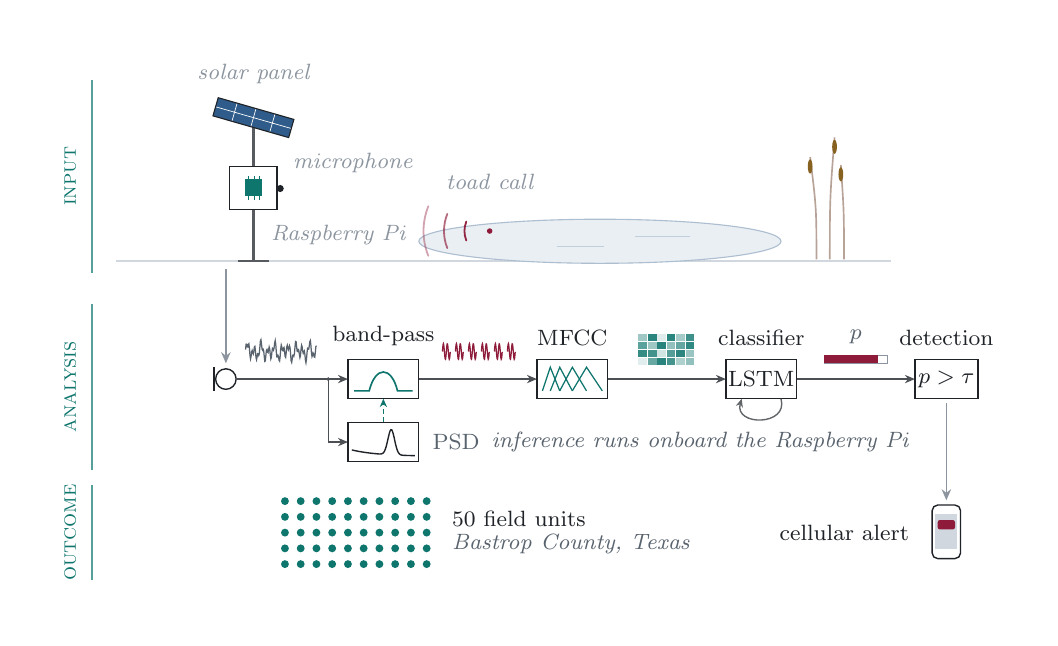
\begin{tikzpicture}[
    font=\footnotesize, text=ink,
    show background rectangle,
    background rectangle/.style={fill=white},
    inner frame sep=10pt,
    tag/.style={text=faint, font=\footnotesize\itshape},
    note/.style={text=mute, font=\footnotesize\itshape},
    region/.style={text=ml, font=\footnotesize\scshape, rotate=90, anchor=south},
    blk/.style={draw=ink, line width=0.5pt, fill=white},
    wire/.style={draw=ink!80, line width=0.55pt, -{Stealth[length=3.6pt, width=3pt]}},
    flow/.style={draw=faint, line width=0.6pt, -{Stealth[length=4pt, width=3.4pt]}}]

  % ----------------------------------------------------------- tiers
  \foreach \ya/\yb/\t in {4.45/6.90/input, 1.95/4.05/analysis, 0.55/1.75/outcome} {
    \draw[ml!70, line width=0.5pt] (-0.05,\ya) -- (-0.05,\yb);
    \node[region] at (-0.13,{(\ya+\yb)/2}) {\t};
  }

  % ------------------------------------------- input: field recording
  \draw[rule, line width=0.5pt] (0.25,4.60) -- (10.10,4.60);
  \draw[ink!75, line width=1.2pt] (2.00,4.60) -- (2.00,6.30);
  \draw[ink!75, line width=0.6pt] (1.80,4.60) -- (2.20,4.60);
  \fill[white] (1.70,5.25) rectangle (2.30,5.80);
  \draw[ink, line width=0.45pt] (1.70,5.25) rectangle (2.30,5.80);
  \fill[ml] (1.89,5.42) rectangle (2.11,5.64);
  \foreach \t in {0.05,0.12,0.19}
    \draw[ml, line width=0.3pt] (1.89+\t,5.42) -- ++(0,-0.04) (1.89+\t,5.64) -- ++(0,0.04);
  \fill[ink] (2.34,5.52) circle (0.045);
  \begin{scope}[shift={(2.00,6.42)}, rotate=-16]
    \fill[slate] (-0.50,-0.12) rectangle (0.50,0.12);
    \draw[white, line width=0.25pt] (-0.25,-0.12) -- (-0.25,0.12) (0,-0.12) -- (0,0.12)
      (0.25,-0.12) -- (0.25,0.12) (-0.50,0) -- (0.50,0);
    \draw[ink, line width=0.4pt] (-0.50,-0.12) rectangle (0.50,0.12);
  \end{scope}
  \fill[slate!10] (6.40,4.85) ellipse[x radius=2.30, y radius=0.28];
  \draw[slate!40, line width=0.4pt] (6.40,4.85) ellipse[x radius=2.30, y radius=0.28];
  \draw[slate!30, line width=0.35pt] (5.85,4.79) -- (6.45,4.79) (6.85,4.91) -- (7.55,4.91);
  \foreach \x/\h/\b in {9.15/1.30/-8, 9.32/1.55/6, 9.50/1.20/-4} {
    \draw[reed, line width=0.6pt] (\x,4.62) .. controls (\x,{4.62+0.5*\h}) .. ({\x+\b*0.01},{4.62+\h});
    \fill[ochre!70!black] ({\x+\b*0.01},{4.50+\h}) ellipse[x radius=0.03, y radius=0.09];
  }
  \foreach \r/\o in {0.32/0.95, 0.58/0.65, 0.84/0.40}
    \draw[call, line width=0.65pt, opacity=\o, line cap=round]
      (5.00,4.98) ++(158:\r) arc[start angle=158, end angle=202, radius=\r];
  \fill[call] (5.00,4.98) circle (0.035);
  \node[tag, anchor=south] at (5.00,5.38) {toad call};
  \node[tag, anchor=south] at (2.00,6.72) {solar panel};
  \node[tag, anchor=south west] at (2.38,5.60) {microphone};
  \node[tag, anchor=north west] at (2.10,5.18) {Raspberry Pi};

  \draw[flow] (1.65,4.50) -- (1.65,3.30);

  % --------------------------------------- analysis: onboard pipeline
  \draw[ink, line width=0.5pt] (1.65,3.10) circle (0.13);
  \draw[ink, line width=0.9pt] (1.50,2.95) -- (1.50,3.25);
  \draw[wire] (1.78,3.10) -- (3.20,3.10);
  \draw[mute, line width=0.45pt] plot[domain=0:0.9, samples=130]
    ({1.90+\x},{3.45+0.07*sin(4100*\x)+0.05*sin(9700*\x+30)+0.04*sin(2300*\x)});
  \fill[ink!80] (2.95,3.10) circle (0.025);
  \draw[ink!80, line width=0.5pt] (2.95,3.10) -- (2.95,2.30);
  \draw[wire] (2.95,2.30) -- (3.20,2.30);

  \draw[blk] (3.20,2.05) rectangle (4.10,2.55);                               % PSD
  \draw[ink, line width=0.5pt] plot[domain=0:0.8, samples=80]
    ({3.25+\x},{2.12+0.32*exp(-pow((\x-0.5)/0.06,2))+0.08*exp(-3*\x)});
  \node[anchor=west, text=mute] at (4.15,2.30) {PSD};
  \draw[ml, line width=0.5pt, dash pattern=on 1.8pt off 1.4pt, -{Stealth[length=3pt, width=2.6pt]}]
    (3.65,2.55) -- (3.65,2.85);

  \draw[blk] (3.20,2.85) rectangle (4.10,3.35);                               % band-pass
  \draw[ml, line width=0.6pt] (3.28,2.95) -- (3.47,2.95) .. controls (3.55,3.27) and (3.75,3.27) .. (3.83,2.95) -- (4.02,2.95);
  \node[anchor=south] at (3.65,3.40) {band-pass};
  \draw[wire] (4.10,3.10) -- (5.60,3.10);
  \foreach \k in {0,...,5}
    \draw[call, line width=0.45pt] plot[domain=0:0.1, samples=24] ({4.40+0.165*\k+\x},{3.45+0.10*sin(7200*\x)});

  \draw[blk] (5.60,2.85) rectangle (6.50,3.35);                               % MFCC
  \foreach \a/\b/\c in {5.67/5.77/5.89, 5.77/5.89/6.05, 5.89/6.05/6.23, 6.05/6.23/6.43}
    \draw[ml, line width=0.45pt] (\a,2.95) -- (\b,3.25) -- (\c,2.95);
  \node[anchor=south] at (6.05,3.40) {MFCC};
  \draw[wire] (6.50,3.10) -- (8.00,3.10);
  \foreach \i in {0,...,5} \foreach \j in {0,...,3} {
    \pgfmathsetmacro\o{0.12+0.78*abs(sin(41*\i+67*\j+13*\i*\j))}
    \fill[ml, opacity=\o] (6.89+0.12*\i,3.28+0.10*\j) rectangle ++(0.11,0.09);
  }

  \draw[blk] (8.00,2.85) rectangle (8.90,3.35);                               % LSTM
  \node at (8.45,3.10) {LSTM};
  \draw[ink!70, line width=0.5pt, -{Stealth[length=3pt, width=2.6pt]}]
    (8.70,2.85) .. controls (8.80,2.50) and (8.10,2.50) .. (8.20,2.85);
  \node[anchor=south] at (8.45,3.40) {classifier};
  \draw[wire] (8.90,3.10) -- (10.40,3.10);
  \draw[faint, line width=0.4pt] (9.25,3.30) rectangle (10.05,3.40);
  \fill[call] (9.25,3.30) rectangle (9.93,3.40);
  \node[anchor=south, text=mute] at (9.65,3.42) {$p$};

  \draw[blk] (10.40,2.85) rectangle (11.20,3.35);                             % decision
  \node at (10.80,3.10) {$p > \tau$};
  \node[anchor=south] at (10.80,3.40) {detection};
  \node[note, anchor=west] at (4.90,2.30) {inference runs onboard the Raspberry Pi};

  \draw[flow] (10.80,2.80) -- (10.80,1.56);

  % ------------------------------------------------ outcome: alerts
  \draw[ink, line width=0.5pt, rounded corners=2pt, fill=white] (10.62,0.82) rectangle (10.98,1.50);
  \fill[rule] (10.66,0.94) rectangle (10.94,1.38);
  \fill[call, rounded corners=0.8pt] (10.69,1.19) rectangle (10.91,1.31);
  \node[anchor=east] at (10.45,1.15) {cellular alert};
  \foreach \i in {0,...,9} \foreach \j in {0,...,4}
    \fill[ml] (2.40+0.20*\i,0.75+0.20*\j) circle (0.05);
  \node[anchor=west, align=left] at (4.40,1.15) {50 field units\\[-1pt]\textcolor{mute}{\itshape Bastrop County, Texas}};
\end{tikzpicture}
\end{document}
